
\begin{frame}{\citetitle{MarcoNuno_CongArbEsp_2014_09_02}$^*$  (1)}
\begin{columns}
\begin{column}{0.6\textwidth}
	\begin{itemize}
		\item El estudiante había trabajado en CAPUFE
        \item Tener un mecanismo que evitara que los vehiculos pagaran menos peaje debido a errores de registro
		\item Contar de manera automática el número de ejes de los vehículos
	\end{itemize}
\end{column}
\begin{column}{0.4\textwidth}  
\begin{center}
     \begin{tabular}{c}
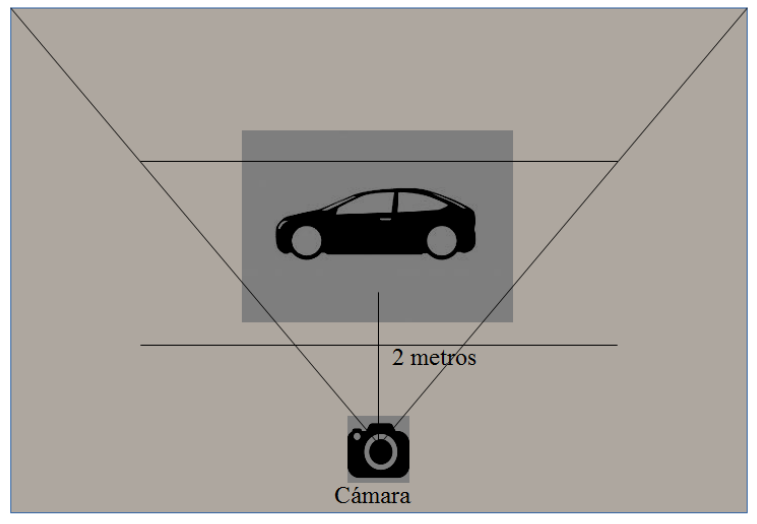
\includegraphics[width=0.68\textwidth]{2014_Llantas/figs/LuisRodolfo1}\\
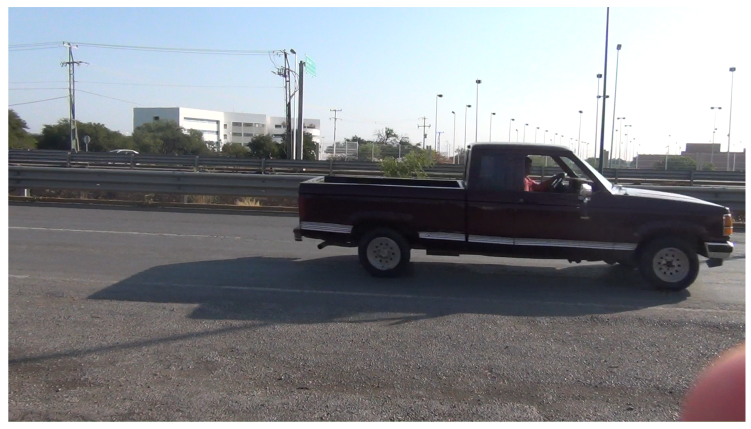
\includegraphics[width=0.68\textwidth]{2014_Llantas/figs/LuisRodolfo2}\\         
      \end{tabular}
\end{center}
\end{column} 
\end{columns} 
\footfullcite*{MarcoNuno_CongArbEsp_2014_09_02}
\end{frame}


\begin{frame}{\citetitle{MarcoNuno_CongArbEsp_2014_09_02} (2)}
	\begin{itemize}
        \item Detectar el vehiculo
        \item Acotar las zonas de interes
        \item Aplicar filtrado a los frames individuales
        \item Detectar contornos para reducir la región de búsqueda de las regiones circulares
        \item Aplicar detección de circulos y generar como resultado el número de ejes
	\end{itemize}
\begin{center}
 \begin{tabular}{cccc}
    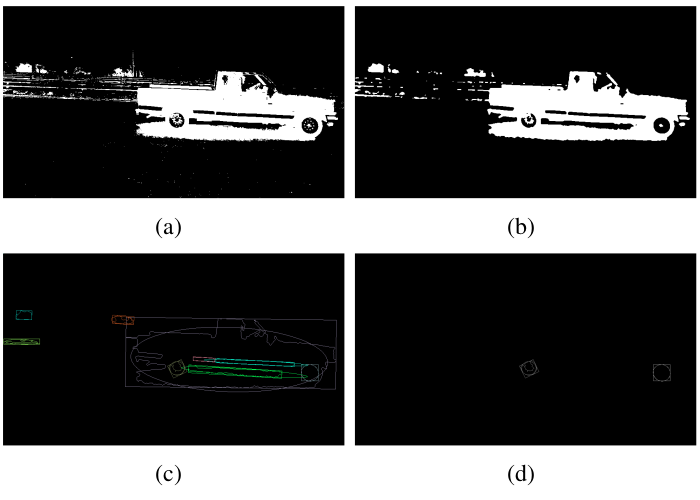
\includegraphics[width=5cm]{2014_Llantas/figs/LuisRodolfo5}
    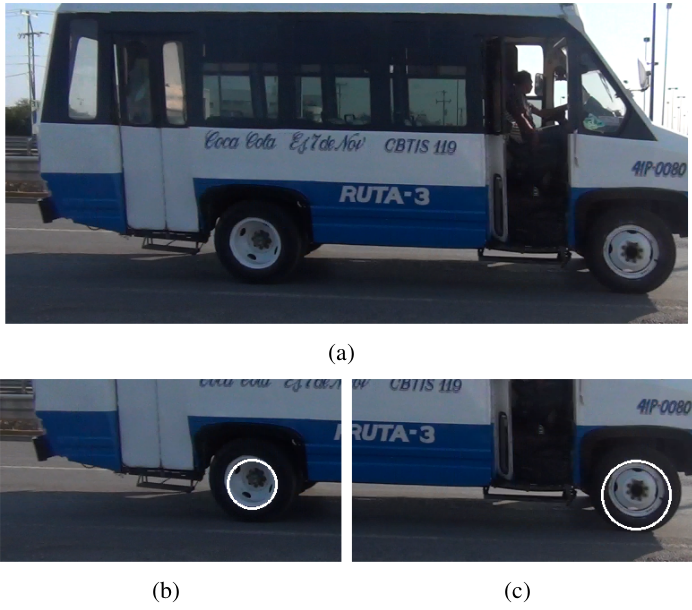
\includegraphics[width=4cm]{2014_Llantas/figs/LuisRodolfo3}
    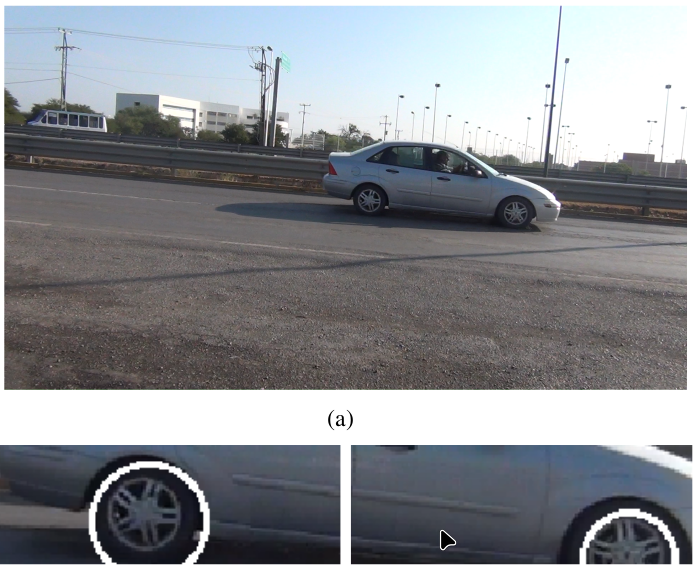
\includegraphics[width=4cm]{2014_Llantas/figs/LuisRodolfo4}
  \end{tabular}
\end{center}

\end{frame}






